%===================================================================================
% Chapter: Results
%===================================================================================
\chapter*{Capítulo 3. Resultados}\label{chapter:results}
\addcontentsline{toc}{chapter}{Capítulo 3. Resultados}
%===================================================================================
\stepcounter{chapter}

\section{Generalidades}
Para iniciar la experimentación fue necesario normalizar los datos y luego se realizaron tres fases de experimentos. En la primera fase se probaron varias arquitecturas de red con el conjunto de datos original. Para la segunda fase se analizó la reducción de dimensiones utilizando el algoritmo de bosques aleatorios. Como última fase se modificó el conjunto de datos original para obtener uno nuevo y probar los algoritmos anteriores.

Como se mencionó anteriormente, es de especial interés medir en cada modelo los casos falsos positivos ($FP$) y falsos negativos ($FN$). En adición se utilizaron las métricas de tasa de aciertos (\textit{accuracy}), 
\[acc = \frac{TP + TN}{TP + FP + TN + FN}\] 
precisión \cite{salton1983introduction} (\textit{precision}), 
\[P = \frac{TP}{TP + FP}\]
 y sensibilidad \cite{allen1955machine} (\textit{recall}). 
\[R = \frac{TP}{TP + FN}\]
Estas métricas son de gran ayuda para comparar diversos resultados en otros trabajos.

\section{Procesamiento de los datos}
El conjunto de datos posee 42 características por cada entrada, las primeras 41 forman parte de la descripción del paquete de red y la última es la clasificación de este. Esta última puede variar, en los archivos con la extensión arff la clase es normal o anómalo, por otro lado, en los archivos txt, si el paquete es de un ataque, se especifica el tipo de ataque. Como se mencionó anteriormente, este documento se centra en la clasificación de los datos en normal y anómalos.

Para el proceso de normalización se investigaron todos los datos en los conjuntos de entrenamiento y de prueba. Las características de cada uno pueden ser de dos tipos, numéricas con valores reales o cualitativas con valores predefinidos. En el caso de las variables numéricas se escalaron todos sus valores al rango [0, 1] buscando el valor mínimo y máximo:
\[A_{i} = \frac{A_{i} - Min_{i}}{Max_{i} - Min_{i}}\] 
donde $i$ es la $i$-\'esima característica, $A_{i}$ es el vector de los valores de la característica de cada dato y $Min_{i}$, $Max_{i}$ son los valores mínimo y máximo de la característica respectivamente. Por otra parte, en las variables cualitativas se le asignó un índice a cada uno de los posibles valores comenzando por el 0, luego para escalarlos se dividió cada uno por la cantidad de posibles valores menos 1 para así obtener los datos en el rango [0, 1]:
\[A_{i} = \frac{index(A_{i})}{len(i) - 1}\]

\section{Modelos básicos}
% arquitecturas de redes simples con el dataset original
% 4x50                  CT-75.1  21T-52.76
% 64-128-64-32-16       CT-75.4  21T-53.25
% 64-128-128-64-32-16   CT-77.91 21T-58
% TODO: escribir el algoritmo aleatorio
Como primera línea base de la investigación se tiene el algoritmo aleatorio. Este clasifica los datos con un 50\% de probabilidad para cada clase sin importar el contenido .Para un acercamiento más al problema y superar los resultados del 50\% del algoritmo aleatorio, se construyeron redes neuronales que entrenaron y evaluaron con el conjunto de datos original. El modelo 1 posee una arquitectura de 4 capas ocultas y cada una con 50 neuronas:
\begin{verbatim}
    from keras import models, layers

    model = models.Sequential()

    # Input - Layer
    model.add(layers.Dense(50, input_dim=(41), 
        activation='relu', name='input_layer'))

    # Hidden - Layers
    model.add(layers.Dropout(0.5))
    model.add(layers.Dense(50, activation='relu', 
        name='hidden_layer_1'))
    model.add(layers.Dropout(0.5))
    model.add(layers.Dense(50, activation='relu', 
        name='hidden_layer_2'))
    model.add(layers.Dropout(0.5))
    model.add(layers.Dense(50, activation='relu', 
        name='hidden_layer_3'))

    # Output - Layer
    model.add(layers.Dense(1, activation='sigmoid', 
        name='output_layer'))
\end{verbatim}

En este modelo, como en los restantes, se utilizó como función de activación en las capaz intermedias ReLU. Por otra parte, en la capa de salida es necesaria la función sigmoide que tiene como resultado valores entre 0 y 1, dado que los datos de entrenamiento fueron modificados y los casos de tráfico anómalo tienen valor 1 y los normales valor 0 en su campo de clasificación, tomando los casos $< 0.5$ como tráfico normal y los $\geq 0.5$ tráfico anómalo.

Como en todos los casos se trabaja con redes neuronales de un tamaño considerable, varios ciclos de entrenamiento y un conjunto de datos con una gran cantidad de entradas, esto puede producir un sobreajuste en las fases de entrenamiento. Como medida de contención se le aplicó la técnica \textit{dropout} a varias capas intermedias de cada uno de los modelos.

\begin{figure}[!hb]
    \centering
    \subfigure{\label{fig:4x5_accuracy}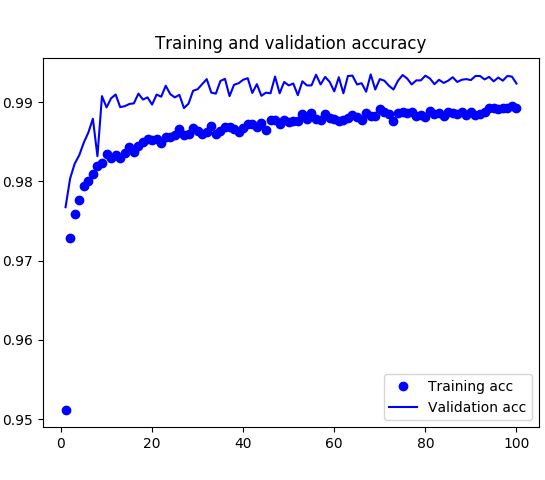
\includegraphics[width=.48\linewidth]{Images/4x50_accuracy.png}}
    \subfigure{\label{fig:4x5_loss}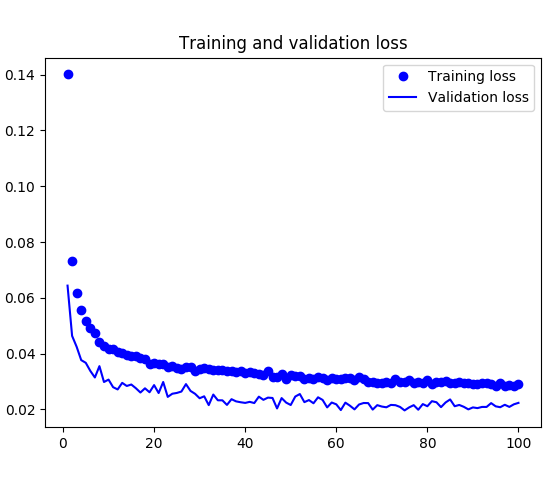
\includegraphics[width=.48\linewidth]{Images/4x50_loss.png}}

    \caption{Tasa de aciertos (\textit{acc}) y pérdida en la fase de entrenamiento del modelo 1 inicial. En el eje X de ambas se muestran los \textit{epochs} y en el eje Y los valores de \textit{acc} y pérdida respectivamente.}
    \label{fig:4x5_train}
\end{figure}

En el proceso de entrenamiento llevado a cabo por cada modelo, se iteraron 100 veces sobre todos los datos(\textit{epochs}) en lotes de tamaño 64(\textit{batch}). Los resultados de la fase de entrenamiento del modelo 1 se pueden observar en la figura \ref{fig:4x5_train}. Para probar los modelos 1, 2 y 3 se utilizaron los dos conjuntos de datos de prueba expuestos en la sección \ref{section:dataset_description}. Como los resultados pueden variar con cada entrenamiento, se realizó este proceso 10 veces y se ejecutaron las pruebas en cada uno, obteniendo 10 resultados que se promediaron para tener un valor m\'as preciso.

Se puede observar que los resultados obtenidos superan al 50\% del algoritmo aleatorio en ambos conjuntos de prueba. A pesar de ello difieren de la fase de entrenamiento lo cual indica que el modelo no está generalizando correctamente los datos. En búsqueda de modelos con mayor comprensión de los datos se crearon dos nuevos, uno con 64, 128, 64, 32 y 16 y el otro con 64, 128, 128, 64, 32 y 16 neuronas en cada capa, en ese orden empezando por la primera capa oculta y terminando en la última respectivamente. Los comportamientos en las fases de entrenamiento fueron similares y los resultados con los conjuntos KDDTest+ y KDDTest-21, junto a los del modelo~1, se pueden observar en las tablas \ref{tab:kddtest+_results} y \ref{tab:kddtest21_results} respectivamente.

\begin{table}[h!b]
    \begin{center}
        \label{tab:kddtest+_results}
        \begin{tabular}{c|c|c|c} % <-- Alignments: 1st column left, 2nd middle and 3rd right, with vertical lines in between
        \textbf{} & \textbf{Modelo 1} & \textbf{Modelo 2} & \textbf{Modelo 3}\\
        \hline
        FP & 232 & 240 & 236\\
        &(1.03\%)&(1.06\%)&(1.05\%)\\
        FN & 5066 & 4966 & 4909\\
        &(22.47\%)&(22.03\%)&(21.77\%)\\
        acc & 0.7649 & 0.7691 & 0.7718\\
        P & 0.9709 & 0.9704 & 0.9711\\
        R & 0.6052 & 0.6130 & 0.6175\\
        \end{tabular}

        \caption{Resultados promedio de los modelos iniciales en el conjunto de prueba KDDTest+.}
    \end{center}
\end{table}

\begin{table}[t]
    \begin{center}
        \label{tab:kddtest21_results}
        \begin{tabular}{c|c|c|c} % <-- Alignments: 1st column left, 2nd middle and 3rd right, with vertical lines in between
        \textbf{} & \textbf{Modelo 1} & \textbf{Modelo 2} & \textbf{Modelo 3}\\
        \hline
        FP & 229 & 234 & 233\\
        &(1.93\%)&(1.97\%)&(1.97\%)\\
        FN & 5066 & 4966 & 4909\\
        &(42.75\%)&(41.91\%)&(41.63\%)\\
        acc & 0.5531 & 0.5612 & 0.5661\\
        P & 0.9529 & 0.9529 & 0.9536\\
        R & 0.4776 & 0.4879 & 0.4938\\
        \end{tabular}

        \caption{Resultados promedio de los modelos iniciales en el conjunto de prueba KDDTest-21.}
    \end{center}
\end{table}

\section{Selección de características}

Para una mejor comprensión de los datos se realizaron múltiples gráficas en las que se muestran una relación de dos de las características y datos de tráfico normal y anómalo. En la mayoría de estas existe una gran dispersión de los datos y no se observa un par de características evidentes que separen al conjunto como se puede observar en \ref{fig:entropy}. Por otra parte, si se observan algunas que aportan muy poca o nada de información, esto se evidencia en \ref{fig:redundant}. En estos casos se tiene la característica $dst\_host\_diff\_srv\_rate$ que en la figura \ref{fig:entropy} si influye en la clasificación de los datos, sin embargo, en \ref{fig:redundant}, cualquiera sea el valor que tome los resultados no varían mucho.

\begin{figure}[b]
    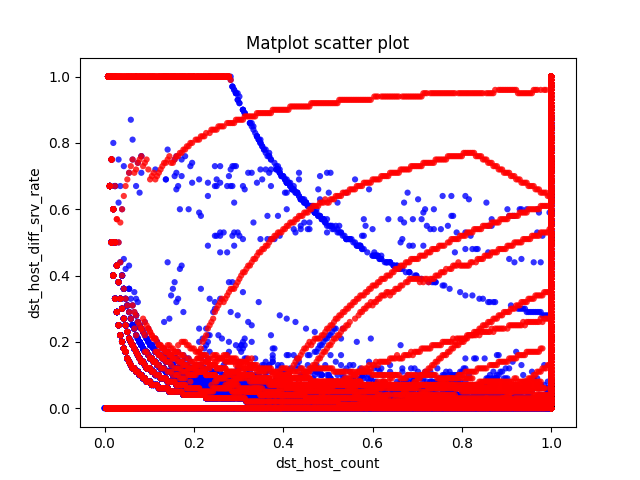
\includegraphics[width=\linewidth]{Images/dst_host_count-dst_host_diff_srv_rate.png}
    \caption{Gráfico que relaciona dos características de los datos. Los puntos rojos son anomalías y los azules tráfico común.}
    \label{fig:entropy}
\end{figure}

\begin{figure}[t]
    \centering
    \subfigure{\label{fig:redundant_a}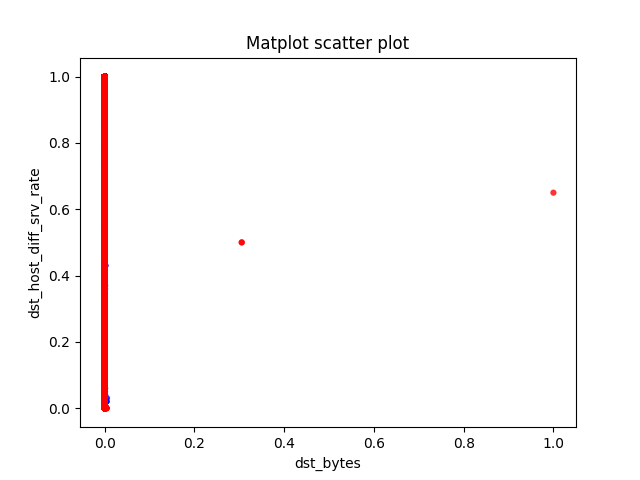
\includegraphics[width=.48\linewidth]{Images/dst_bytes-dst_host_diff_srv_rate.png}}
    \subfigure{\label{fig:redundant_b}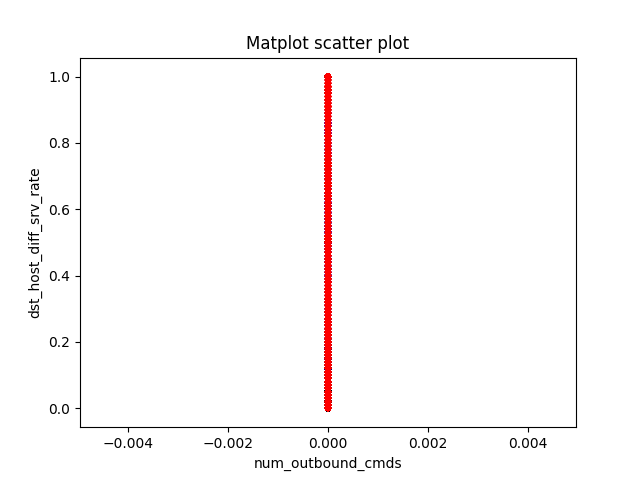
\includegraphics[width=.48\linewidth]{Images/num_outbound_cmds-dst_host_diff_srv_rate.png}}

    \caption{Característica que aportan muy poca información en la clasificación de los datos.}
    \label{fig:redundant}
\end{figure}

Las características redundantes hacen que a los modelos les tome más tiempo llevar a cabo la fase de entrenamiento o pueden causar un sobreajuste (\textit{overfitting}) que puede afectar la generalización, entre otros problemas \cite{tuv2009feature}. Como se explicó anteriormente, el algoritmo de bosques aleatorios basa su funcionamiento en la importancia de las características por lo que es de gran utilidad para saber la utilidad de cada una. Para esto se entrenó y probó el algoritmo con varios parámetros, 10 veces en cada ocasión y se promediaron los resultados. La métrica usada en este caso fue el \textit{accuracy} y ofreció los valores 0.7618 y 0.5469 para los conjuntos KDDTest+ y KDDTest-21 respectivamente con los parámetros que se muestran a continuación:

\begin{verbatim}
    parameters = {
    # Activa la toma de muestras aleatorias con reemplazo
    'bootstrap': True,

    # Mínimo numero de ejemplos para considerar un nodo hoja
    'min_samples_leaf': .001, # representa el 0.1% del dataset

    # Número de árboles en el bosque
    'n_estimators': 100,

    # Número mínimo de ejemplos para dividir un nodo interno
    'min_samples_split': 20,

    # Numero de características a considerar cuando se busca 
    la mejor división
    'max_features': 20,

    # Máxima profundidad de los árboles
    'max_depth': 6,

    # Número máximo de nodos hojas. Si es none la cantidad de 
    hojas es ilimitados
    'max_leaf_nodes': None
}
\end{verbatim}

Los resultados obtenidos con los bosques aleatorios son bastante similares a los brindados por los primeros modelos, al igual que a los de algunas bibliografías \cite{abualkibash2019machine}, por lo que este algoritmo está analizando bien los datos. Después se procedió a extraer la importancia de las características. Los resultados para los conjuntos KDDTrain+ y KDDTest+ se muestra en las figuras \ref{fig:features_relevance_train} y \ref{fig:features_relevance_test} respectivamente.

\begin{figure}[h!t]
    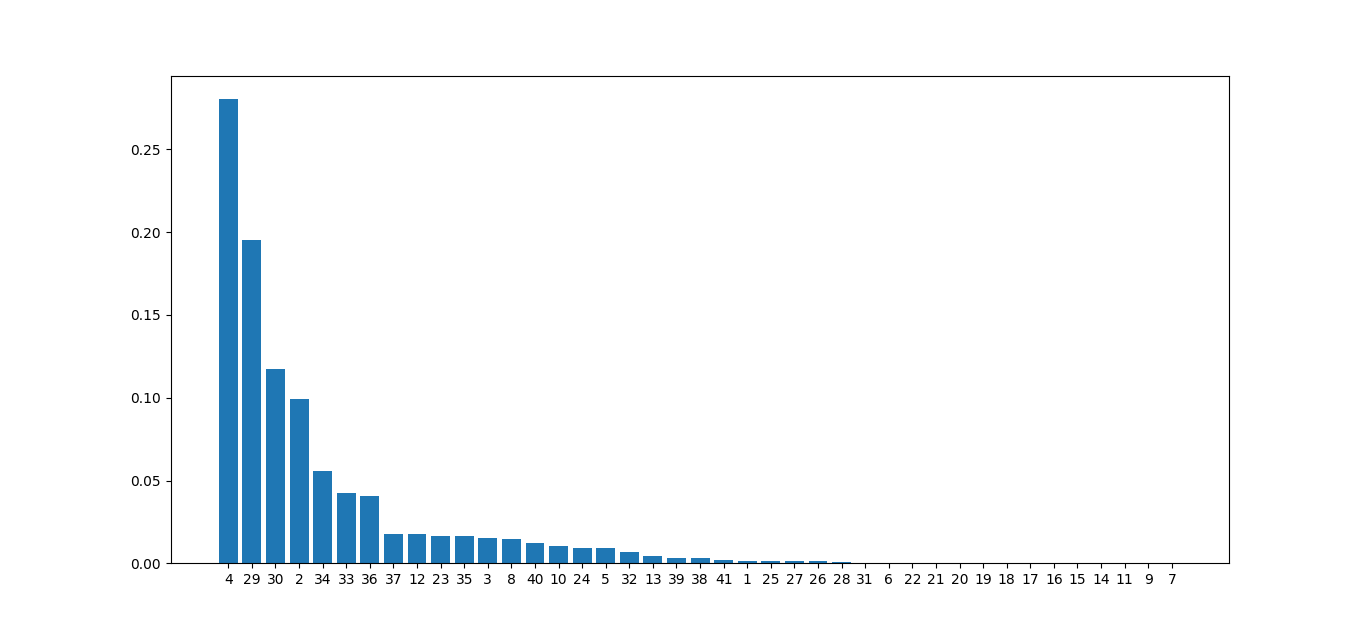
\includegraphics[width=\linewidth]{Images/features_relevance_train.png}
    \caption{Importancia de cada característica en el conjunto KDDTrain+.En el eje de las X los identificadores de cada característica y en el eje de las Y la importancia.}
    \label{fig:features_relevance_train}
\end{figure}

\begin{figure}[t]
    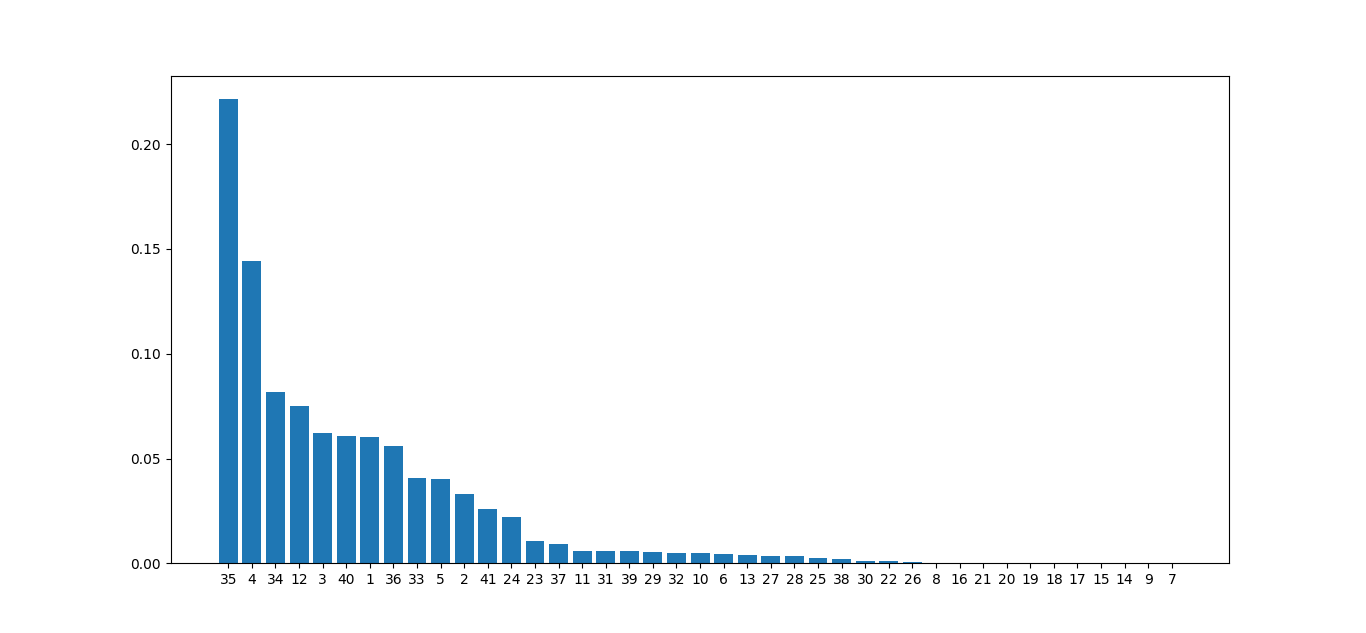
\includegraphics[width=\linewidth]{Images/features_relevance_test.png}
    \caption{Importancia de cada característica en el conjunto KDDTest+. En el eje de las X los identificadores de cada característica y en el eje de las Y la importancia.}
    \label{fig:features_relevance_test}
\end{figure}

Como se puede observar hay características que aportan muy poca o ninguna información. Por este motivo se decidió eliminar de las fases de entrenamiento y prueba las características con identificadores 7, 9, 14, 15, 16, 17, 18, 19, 20, 21 y 22, dejando solo 30 de las 41 existentes. Con esta forma nueva del conjunto de datos se procedió a entrenar y probar los modelos~1,~2~y~3. Los resultados se pueden observar en la tabla \ref{tab:lessfeatures_results}. Como se puede apreciar las diferencias en los resultados no son notables.

\begin{table}[t]
    \begin{center}
        \label{tab:lessfeatures_results}
        \begin{tabular}{c|c|c|c} % <-- Alignments: 1st column left, 2nd middle and 3rd right, with vertical lines in between
        \textbf{} & \textbf{Modelo 1} & \textbf{Modelo 2} & \textbf{Modelo 3}\\
        \hline
        FP & 232 & 231 & 233\\
        &(1.03\%)&(1.02\%)&(1.03\%)\\
        FN & 5061 & 4963 & 5047\\
        &(22.45\%)&(22.01\%)&(22.39\%)\\
        acc & 0.7652 & 0.7696 & 0.7658\\
        P & 0.9710 & 0.9714 & 0.9710\\
        R & 0.6056 & 0.6133 & 0.6067\\
        \hline
        FP & 227 & 225 & 227\\
        &(1.92\%)&(1.90\%)&(1.92\%)\\
        FN & 5061 & 4963 & 5047\\
        &(42.71\%)&(41.88\%)&(42.59\%)\\
        acc & 0.5537 & 0.5622 & 0.5550\\
        P & 0.9532 & 0.9546 & 0.9535\\
        R & 0.4781 & 0.4882 & 0.4796\\
        \end{tabular}

        \caption{Resultados promedio de los modelos en los conjuntos de prueba KDDTest+ (arriba) y KDDTest-21 (abajo) con 30 características en los datos.}
    \end{center}
\end{table}

\subsection{Validación por partes}

% \begin{center}
%     \begin{psmatrix}[rowsep=1cm,colsep=.3cm]
%         & [name=comienzo,mnode=oval] \parbox{3cm}{\centering $(k, S, modelo)$} \\
%         & [name=initP,mnode=circle] $P$ \\
%         & [name=initR,mnode=circle] $R$ \\
%         & [name=initI,mnode=circle] $i$ \\
%         & [name=eval] \psframebox{\parbox{4cm}{\centering
%             $P=\frac{|S|}{k}$ \newline
%             $R = \{\}$ \newline
%             $i = 0$}} \\
%         & [name=if,mnode=dia] $i = k$ &
%         [name=finprog] \psframebox{\parbox{4cm}{\centering Retornar $\frac{\sum{R}}{k}$}} \\
%         & [name=valtrain] \psframebox{\parbox{4cm}{\centering
%             $V = S[i*P ... (i+1)*P]$ \newline
%             $T = S - V$}} \\
%         & [name=recurre] \psframebox{\parbox{4cm}{\centering
%         Entrenar modelo con $T$ \newline
%         Validar modelo con $V$ \newline
%         $R = R +$ resultados de la validaci\'on \newline
%         $i = i + 1$}} \\
        
%         \ncline{->}{comienzo}{initP}
%         \ncline{->}{initP}{initR}
%         \ncline{->}{initR}{initI}
%         \ncline{->}{initI}{eval}
%         \ncline{->}{eval}{if}
%         \ncline{->}{if}{finprog}\naput{Sí}
%         \ncline{->}{if}{valtrain}\naput{No}
%         \ncline{->}{valtrain}{recurre}
%         \ncangle[angleA=180,armB=2cm,angleB=180]{->}{recurre}{if}
%     \end{psmatrix}
% \end{center}

\begin{figure}[h!t]
    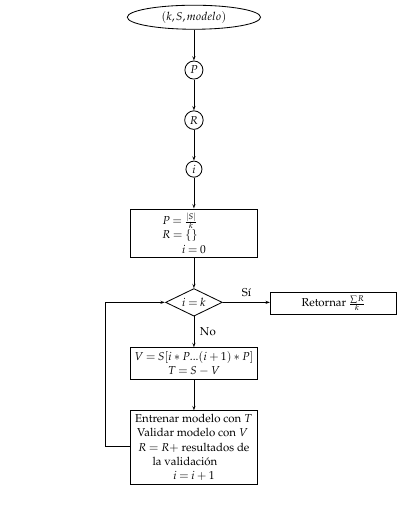
\includegraphics[width=\linewidth]{Images/k_fold.png}
    \caption{Diagrama de flujo para el algoritmo \textit{k-fold}.}
    \label{fig:k_fold}
\end{figure}

Para obtener una mayor confianza en los resultados obtenidos se le aplicó el método de \textit{k-fold} al proceso de aprendizaje. En la etapa de validación se escoge un subconjunto de los datos de entrenamiento por lo que el resultado puede variar bastante dependiendo de la selección, para evitarlo se utiliza \textit{k-fold}. Este consiste en al partición del conjunto de entrenamiento en $k$ pedazos de aproximadamente mismo tamaño. El proceso de aprendizaje se realiza $k$ veces y en la i-\'esima iteración se toma la partición $i$ como conjunto de validación y las $k - 1$ restantes para entrenar el modelo. Una vez terminando se tienen $k$ resultados, estos se promedian y se obtiene una mejor aproximación de la fase de entrenamiento. Este proceso se puede observar en la figura \ref{fig:k_fold}. El valor escogido para $k$ en este caso fue 5 (usualmente se trabaja con 4 o 5). Los resultados promedio, para el modelo 3, de las 5 fases de validación se pueden observar en la tabla \ref{tab:kfold_results}.

\begin{table}[t]
    \begin{center}
        \label{tab:kfold_results}
        \begin{tabular}{c|c|c|c|c|c} % <-- Alignments: 1st column left, 2nd middle and 3rd right, with vertical lines in between
        \textbf{Pérdida} & \textbf{FP} & \textbf{FN} & \textbf{acc} & \textbf{P} & \textbf{R}\\
        \hline
        0.0239 & 39 & 204 & 0.9904 & 0.9966 & 0.9826\\
        &(0.15\%) & (0.81\%) &&&\\
        \end{tabular}

        \caption{Resultados promedio del modelo 3 utilizando el algoritmo de \textit{k-fold} para $k = 5$.}
    \end{center}
\end{table}

% [2.38524386e-02, 9.90370727e-01, 2.03800000e+02, 3.88000000e+01,
%        9.96655357e-01, 9.82594657e-01]

\section{Transformación del conjunto de datos}

\begin{figure}[b]
    \begin{verbatim}
        C <- Train + Test
        desordenar_aleatorio(C)
    
        particion = longitud(C) / 5
    
        nuevo_train = C[todos los datos desde particion 
            hasta el final]
        nuevo_test = C[todos los datos desde el principio 
            hasta particion]
    \end{verbatim}
    \caption{Algoritmo para la creación de los nuevos conjuntos de entrenamiento y de prueba.}
    \label{fig:partition}
\end{figure}

En la sección anterior se pudo observar como los modelos tenían buenos valores en las fases de aprendizaje (\ref{fig:4x5_train}) y sin embargo, en las fases de prueba no tenían la misma efectividad. Esto es un indicador de una mala generalización, o sea, los modelos aprenden muy bien a identificar los datos de entrenamiento pero cuando se enfrentan a datos nuevos no los clasifican con la misma precisión. Al observar la tabla \ref{tab:atk_counts}, es fácil percatarse que los modelos van a tener mayor dificultad a la hora de clasificar ciertos datos, dado que los ataques de tipo \textit{U2R} y \textit{R2L} poseen muchos mas ejemplos en el conjunto de prueba que en el de entrenamiento. 

Por lo mencionado en la sección \ref{section:modified_dataset} se decidió unificar el conjunto KDDTrain y KDDTest, esparcir los datos de forma aleatoria y crear a partir de este nuevo conjunto uno de entrenamiento y otro de prueba. Los datos de entrenamiento nuevos representan el 80\% y los de prueba el 20\%. Al realizar este proceso de forma aleatoria, existe una alta posibilidad en la que los datos pertenecientes a cada tipo de ataque tengan cantidades en los dos conjuntos que mantengan la proporción 80/20. Esto garantiza que los modelos aprendan mejor el comportamiento de algunos datos antes de clasificarlos. El algoritmo de creación de los nuevos conjuntos se puede observar en la figura \ref{fig:partition}.

Dado que el modelo 3 presentó pequeñas mejoras sobre los demás, estas pruebas se realizaron solo con este. El proceso de aprendizaje fué similar a los anteriores y los resultados obtenidos se muestran en la tabla \ref{tab:newdataset_results}. Como se puede observar los resultados son evidentemente superiores, con valores de efectividad de casi un 100\%.

\begin{table}[t]
    \begin{center}
        \label{tab:newdataset_results}
        \begin{tabular}{c|c|c|c|c} % <-- Alignments: 1st column left, 2nd middle and 3rd right, with vertical lines in between
        \textbf{FP} & \textbf{FN} & \textbf{acc} & \textbf{P} & \textbf{R}\\
        \hline
        168 & 294 & 0.9844 & 0.9882 & 0.9794\\
        (0.6\%) & (1\%) &&&\\
        \end{tabular}

        \caption{Resultados promedio del modelo 3 utilizando los conjuntos de entrenamiento y de prueba nuevos, creados a partir de la unión de los anteriores.}
    \end{center}
\end{table}
% [4.50945967e-02 9.84429175e-01 2.94400000e+02 1.68100000e+02 9.88181365e-01 9.79385948e-01]

% k-fold validation
% búsqueda del learning rate

% TODO: demostrar o probar porque con el dataset transformado no es necesario volver a probar los primeros modelos que eran mas malos con el dataset original